\documentclass[11pt,a4paper]{article}
\usepackage[left=2cm,text={17cm,25cm},top=2cm]{geometry}
\usepackage[T1]{fontenc}
\usepackage[czech]{babel}
\usepackage[utf8]{inputenc}
\usepackage{url}
\usepackage{graphicx}
\usepackage{pdfpages}
\usepackage{algorithmicx}
\graphicspath{ {img/} }

\begin{document}

\begin{center}
	\LARGE{Paralelní a distribuované algoritmy -- dokumentace k projektu 3}\\
	\large{Vysoké učení technické v Brně}
	\vspace{0.2cm}

	Petr Stehlík <xstehl14@stud.fit.vutbr.cz>     \today

\end{center}

\section{Zadání}

Cílem projektu byla implementace algoritmu \textit{mesh multiplication}, který byl prezentován během přednášek. Běh a kompilace programu je zprostředkován pomocí skriptu \texttt{test.sh}. Implementace využívá knihovny Open MPI.

\section{Rozbor a analýza algoritmu}

Mesh multiplication je algoritmus pro součin dvou matic $A(m,n)$ a $B(n,k)$, kde výsledkem je matice $C (m,k) = AB$, kde $C_{ij} = \sum\limits_{s=1}^n a_{is} * b_{sj}$, kde $1 \leq i \leq m, 1 \leq j \leq k$. Algoritmus pro jednoznačnost budeme analyzovat na čtvercových maticích, avšak algoritmus je aplikovatelný i na obdélníkové matice jak jsou definovány výše.

Procesory jsou propojeny v dvourozměrné mřízce a lineárně spojeny se svými nejbližšími sousedy. Schéma zapojení procesorů je znázorněné na obrázku \ref{schema}. Na procesory v prvním sloupci a prvním řádku jsou přiváděny prvky matic A a B. Každý procesor obsahuje 3 registry: \textit{C} -- obsahuje výsledek a při inicializaci je nastaven na $0$, \textit{A} -- postupně prvky daného řádku z matice A, \textit{B} -- postupně prvky daného sloupce z matice B. Každý procesor následně posílá prvek z registru A svému pravému sousedovi a prvek z registru B svému spodnímu sousedovi.

\begin{figure}[h]
    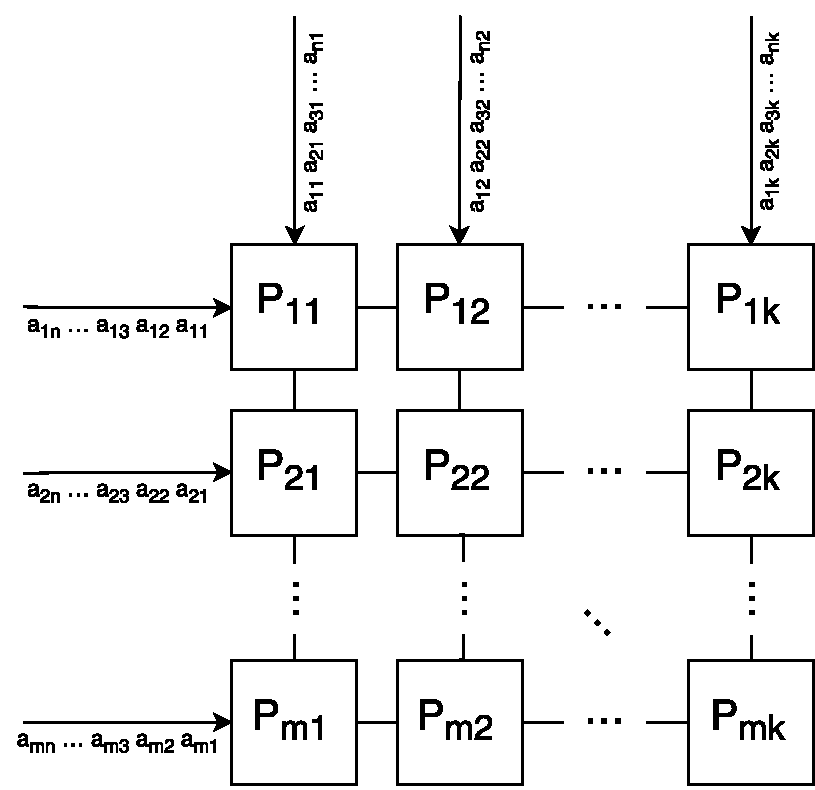
\includegraphics[width=0.4\linewidth]{mesh}
    \centering
	\caption{Schéma zapojení procesorů do mřížky.}
    \label{schema}
\end{figure}

\subsection{Analýza algoritmu}
Nulování registru \textit{C} proběhne v konstatním čase. Poslání prvků $a_{m1}$ a $b_{1k}$ topologicky nejvzdálenějšímu procesoru $P_{mk}$ trvá $m+k+n - 2$ kroků. Pokud předpokládáme, že $m \leq n$ a $k \leq n$, poté má algoritmus časovou složitost $t(n) = \mathcal{O}(n)$. Pokud budeme uvažovat čtvercové matice, bude algoritmus potřebovat celkem $n^2$ procesorů. Z toho vyplývá celková cena algoritmu $c(n) = \mathcal{O}(n^3)$. To značí, že algoritmus mesh multiplication není optimální.

\section{Implementace}

Při inicializaci program vytvoří $m*k$ procesorů, kde procesor $P_{11}$ řídí vstup a výstup programu, rozesílá načtené matice dalším procesorům a vypisuje vypočítanou matici. Načtené matice $A$ a $B$ jsou zkontrolovány, zda jsou v korektním formátu a mohou být spolu vynásobeny a následně jsou jednotlivé řádky matice $A$ poslány na procesory v prvním sloupci a jednotlivé sloupce matice $B$ rozeslány na procesory v prvním řádku. Ty postupně odebírají prvky z fronty a po načtení jednoho prvku z obou matic jsou vynásobeny a přičteny k registru $C$.

Všechny procesory jsou informovány o celkových rozměrech obou matic $A$ a $B$ pomocí \textit{broadcast} zpráv. Pokud při kontrole matic dojde k chybě, je tato chyba také distribuována pomocí \textit{broadcast} zprávy a procesory jsou ukončeny s nenulovým návratovým kódem.

Dále jsou prvky poslány svým pravým a spodním sousedům. Prvky A svým pravým sousedům a prvky B svým spodním sousedům. Procesory na pravém a spodním okraji po výpočtu prvky zahazují.

Po dokončení výpočtu výsledné matice jsou výsledky umístěny v registru $C$. Všechny procesory odešlou prvek v registru $C$ prvnímu procesoru, který prvky ve správném pořadí a formátu vytiskne na standardní výstup. Následně jsou uvolněny všechny alokované zdroje, je provedena finalizace a program je ukončen.

\section{Experimentální ověření časové složitosti}

Experimety probíhaly na stroji disponujícím Intel Core i7-2635QM @ 2.00GHz, 8 GB RAM a SSD. Průměrná doba běhu algoritmu je průměr doby běhu každého z procesorů. Každá konfigurace byla spuštěna desetkrát a z výsledných časů je vybráno maximum, minimum a spočítán aritmetický průměr. Čas výpočtu byl měřen pomocí Open MPI funkce \texttt{Wtime()}. Čtvercové matice pro výpočet byly náhodně generované (s rozsahem čísel od -127 do 128) pomocí knihovny NumPy pro jazyk Python. Z naměřených výsledků je patrné, že pro $n < 15$ je výpočet lineární s relativně malým vlivem režie procesoru a samotných operací násobení a sčítání. Při větších maticích se již znatelně projevuje režie fyzického procesoru.

\begin{figure}[!ht]
    \centering
		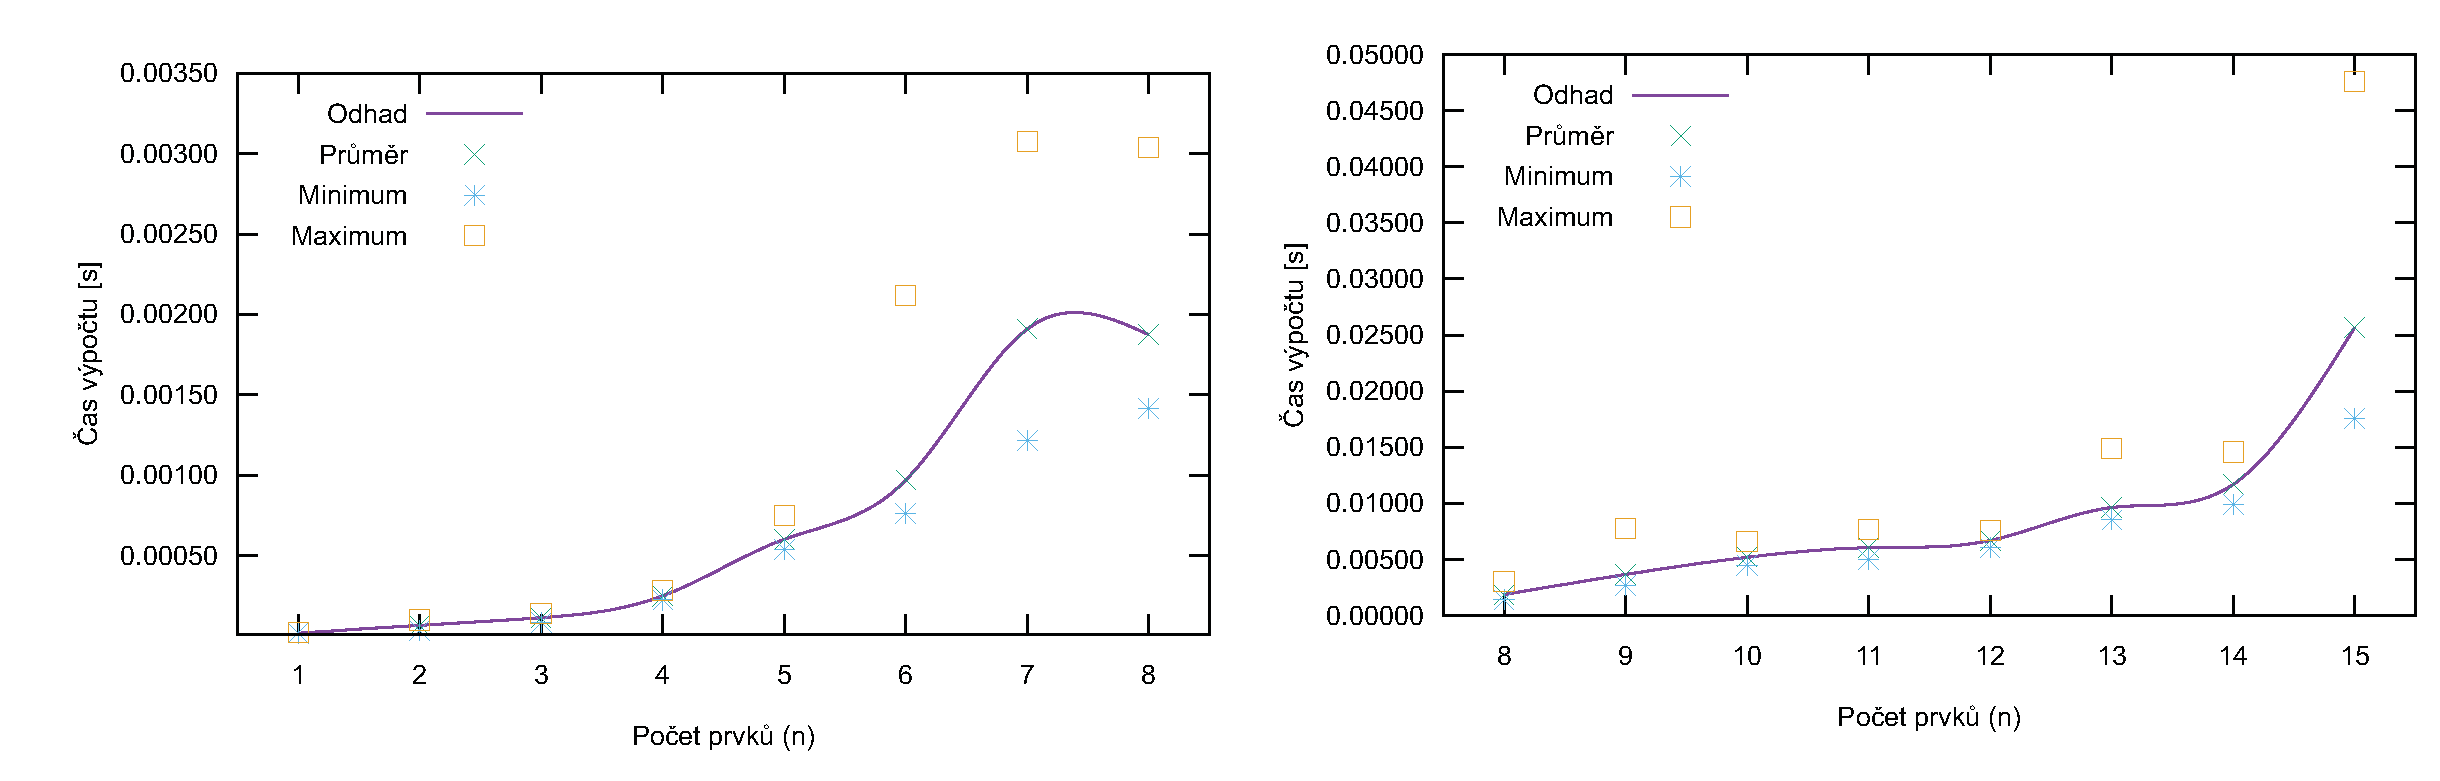
\includegraphics[width=1\textwidth]{results}
    \caption{Experimentálně naměřené výsledky}
\end{figure}

\section{Komunikační protokol}
\label{proto}

Protokol je znázorněn na obrázku \ref{proto_schema}. Zasílání zpráv je realizováno funkcemi \texttt{Send}, \texttt{Isend}, \texttt{Recv} a \texttt{Broadcast} z knihovny Open MPI. Tagy \texttt{ROW} a \texttt{COL} slouží pro zasílání čísel sousedským procesorům, tag \texttt{RES} je označení pro přenos výsledného prvku matice prvnímu procesoru. Dále jsou použity \texttt{Broadcast} zprávy pro zaslání velikosti matic a pro oznámení chyb v programu. Tag \texttt{TIME} je určen pro zasílání výpočetního času daného procesoru prvnímu procesoru.

Broadcast zprávy nejsou zahrnuty v diagramu kvůli přehlednosti. Jejich iniciátorem je vždy první procesor. Program obsahuje následující broadcast zprávy:

\begin{itemize}
    \item{error -- signalizace chyby vykonávání programu nenulovou hodnotou,}
    \item{dim1 -- rozměry matice $A$,}
    \item{dim2 -- rozměry matice $B$.}
\end{itemize}

\begin{figure}[!h]
    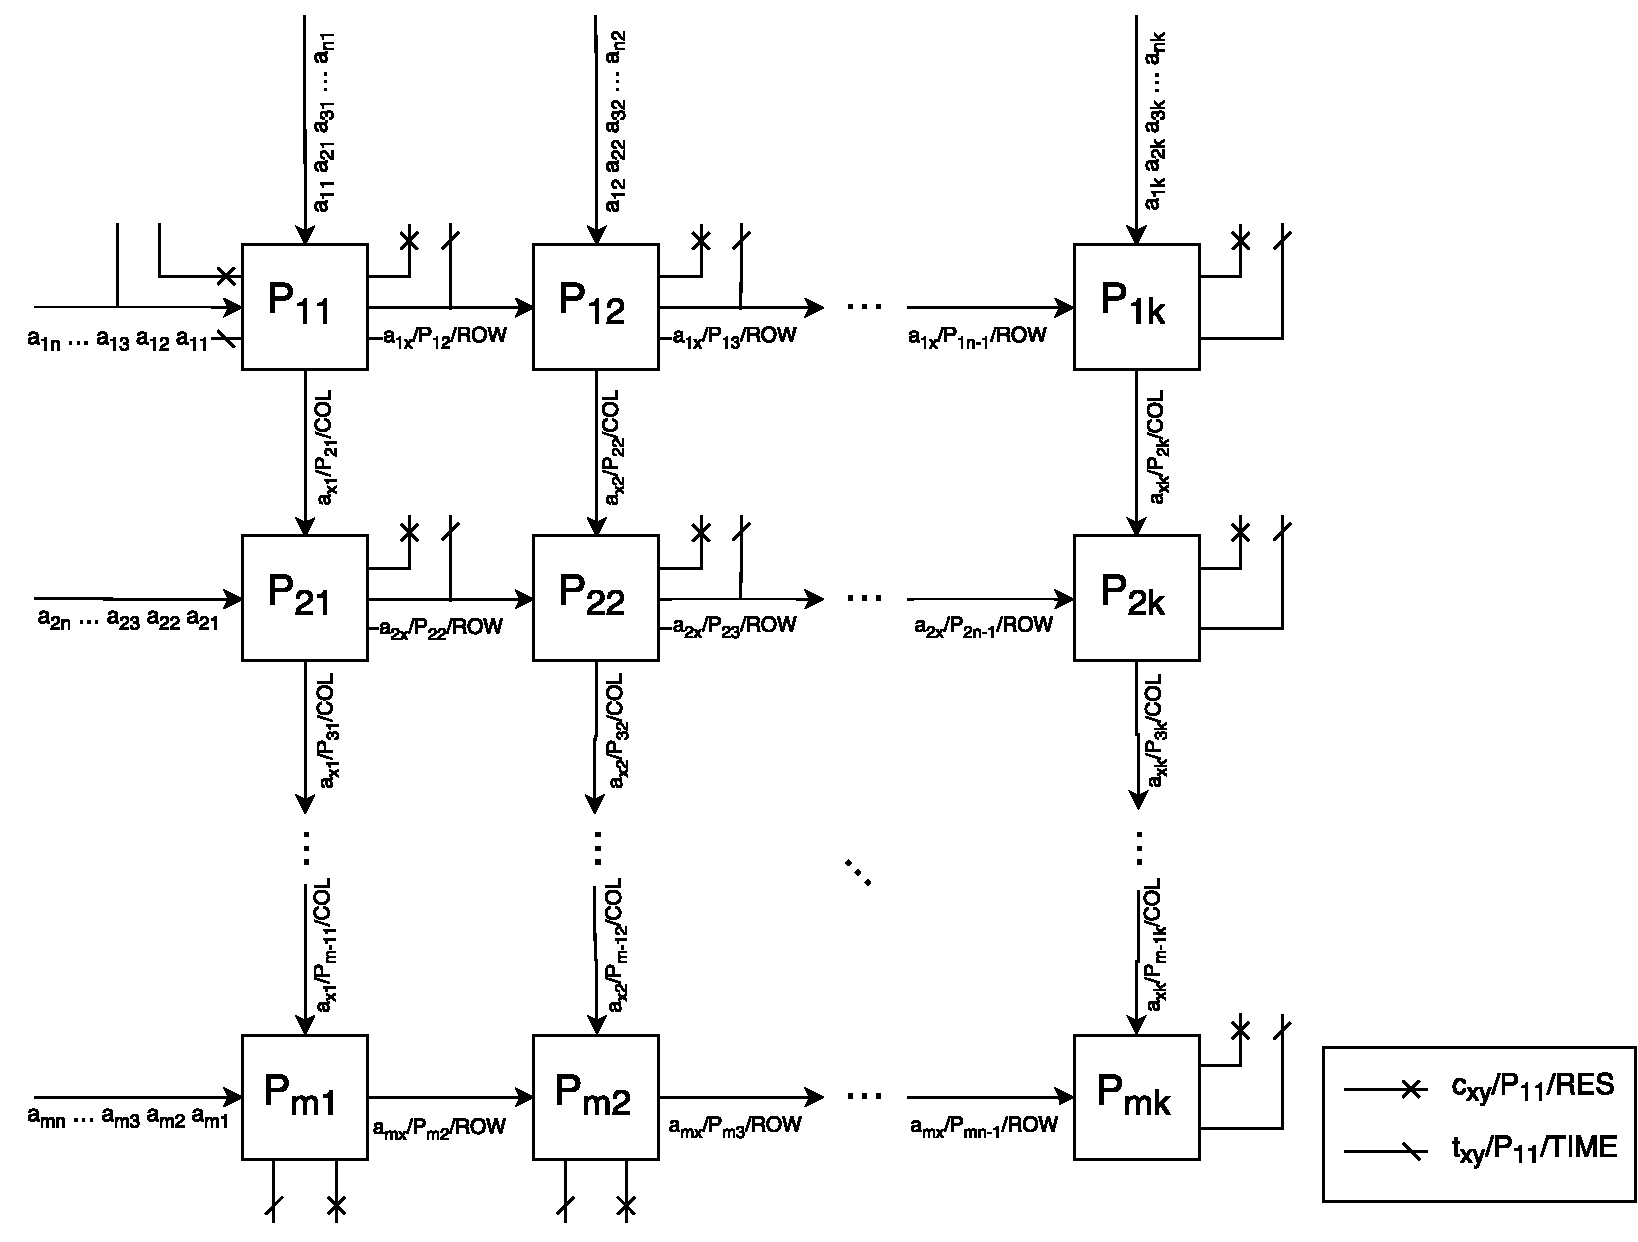
\includegraphics[width=1\linewidth]{protokol}
    \centering
    \caption{Diagram komunikačního protokolu. Popisky obsahují následující informace: zasílaná hodnota/rank/tag.}
    \label{proto_schema}
\end{figure}


\section{Závěr}

Algoritmus \textit{mesh multiplication} se podařilo úspěšně implementovat a experimentálně otestovat. Byla odvozena jeho teoretická časová složitost a cena. Experimenty nad reálnými daty dokazují, že v praxi se algoritmus také blíží lineární časové složitosti s přihlédnutím na režii fyzického procesoru. Experimenty s $n > 14$ těmto předpokládům neodpovídají kvůli vysoké režii při přepínání procesů.

\end{document}

